\section{Intensity Reconstruction}
\subsection{Absolute Intensity in the DVS circuit}

\subsection{BSDF Lighting Model}

\subsection{Additional Bias Currents}

Besides the contrast threshold, other biases are suitable for intensity measurements. The \textit{photo receptor gain} amplifies the voltages generated by the photo receptor. The source follower bandwidth regulates the speed at which the source follower - which sits between the photo receptor and the comparator in the DVS circuit, determines how fast it reacts to intensity changes. Both the photo receptor gain and source follower bias affect the amplitude that the source follower reaches during the short on-duration of the projector pixel it observes.
\newline
\newline
We have found the photoreceptor gain to offer both the highest dynamic range and the highest measurement resolution of the three.
\newline \newline

\section{Depth Reconstruction}

\subsection{Hole Reconstruction}
\begin{figure}
    \centering
    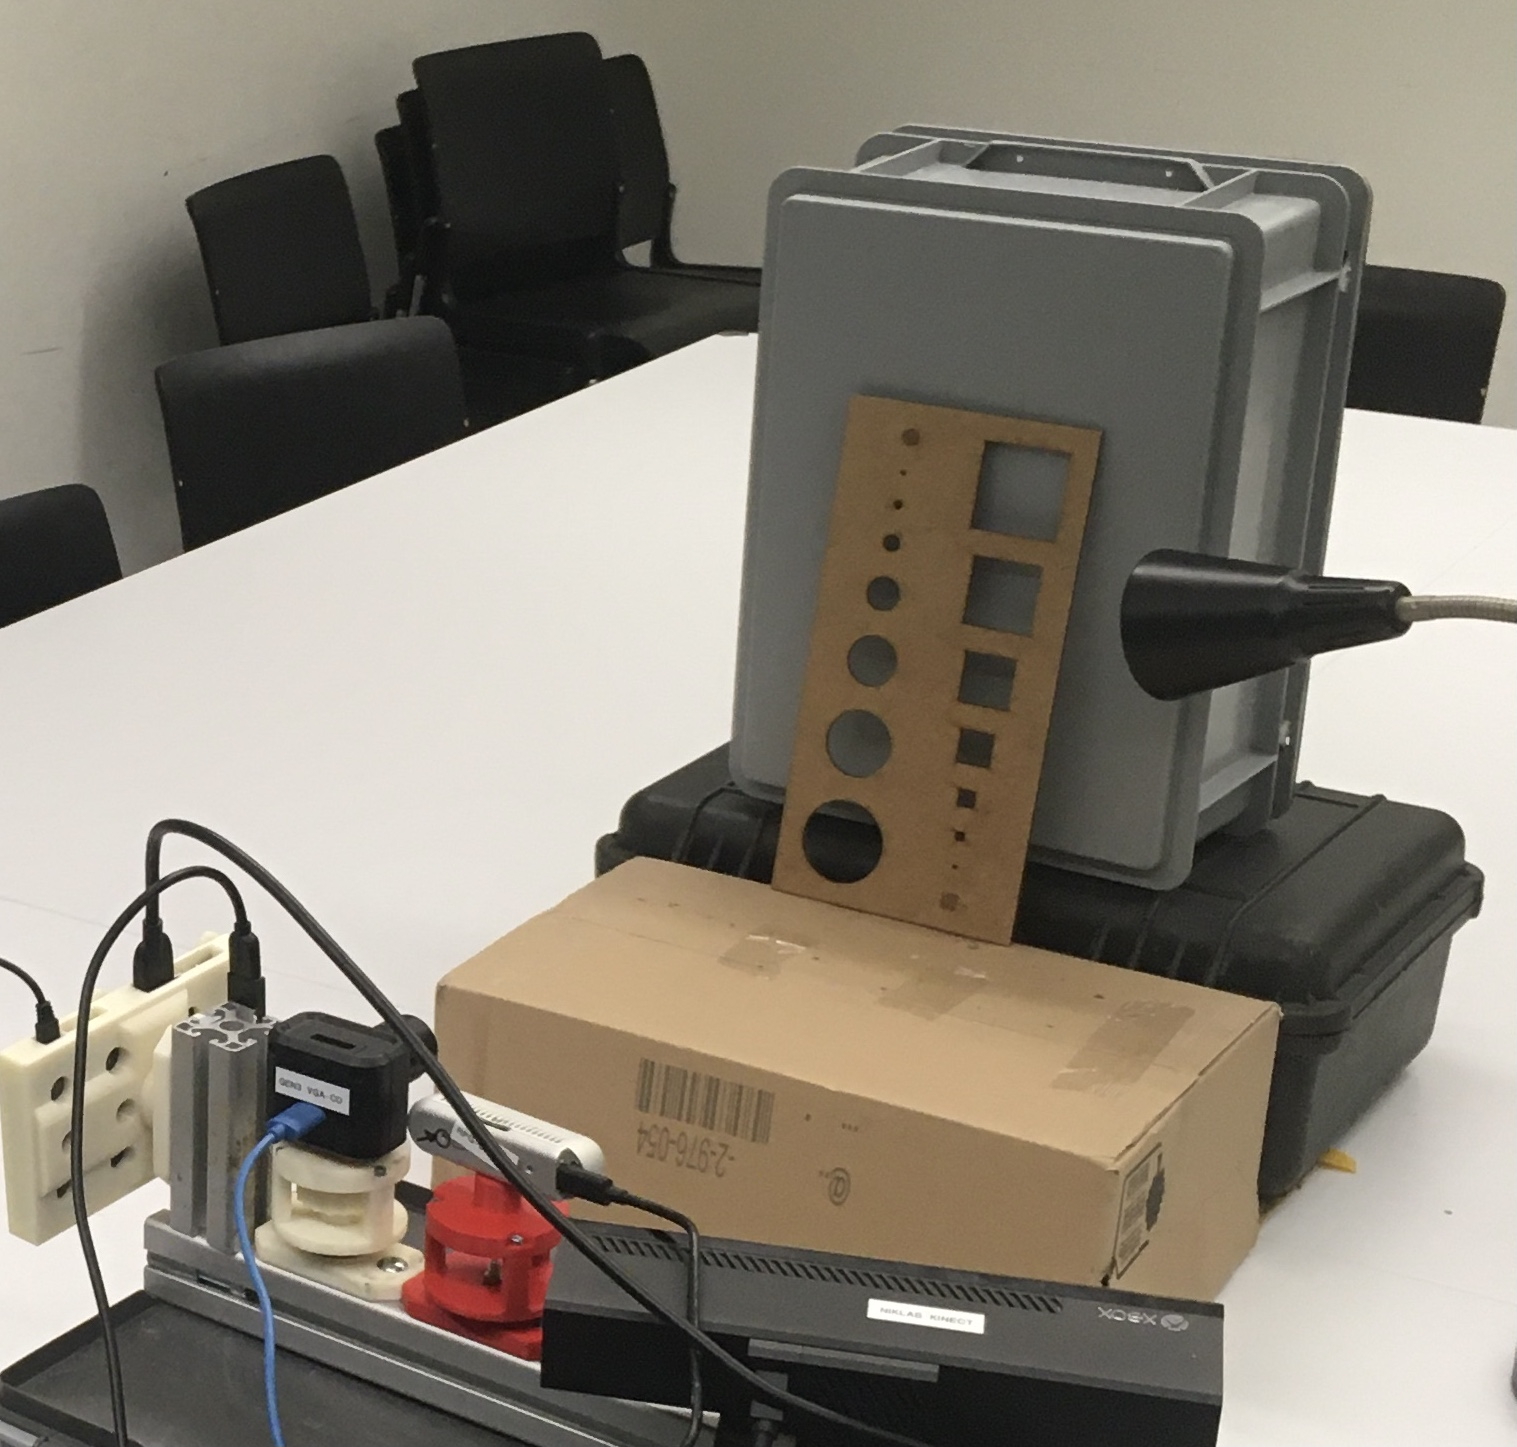
\includegraphics[width=.5\textwidth]{resources/images/depth_estimation/hole_board/setup.jpeg}
    \caption[Image of the Hole Board]{Setup used to capture the ole board with all sensors}
    \label{fig:holeBoardSetup}
\end{figure}
In the previous section, I attempted to measure thin, detailed rods and fence, but our ground-truth method was unable to capture them. As an alternative, I quantify the capabilities of each sensor to measure detail by their ability to capture holes of decreasing size. The laser scanner was able to capture these accurately and there is CAD data available for the laser-cut board I used.
\newline
\newline
The accuracy of small holes would not be represented well by any of the metrics used in the overall point-cloud evaluation and is thus measured here using an Intersection over Union for each hole separately.
I have accurate ground-truth data from the SVG file that was used to cut the holes and thus use this for comparison. The Faro measurements are presented as an additional sensor.
To compare them, the point clouds of the whole board are first aligned and then trimmed in the front and back (respectively 7 and 4 mm are kept in the front and back).
The point clouds are then projected orthographically as circles onto the image plane. 
Finally, sections that are left white (i.e. holes) are compared with the ground truth using an Intersection over Union metric.\\
The trimming is necessary for two reasons: First, the board was leaned against a wall which needs to be removed. Second, the Intel Realsense did not produce any holes, but rather just indentations in a continuous surface. Trimming reveals sufficiently large indentations as holes.\\ It is also important to note that the circles used to draw each point are quite large\footnote{For reference, single points are drawn underneath the scale in the Appendix.}, which reduces the size of each hole and completely fills the smallest 2mm hole. The size of the circles is set such that the reconstruction of the pico flexx2, which has the smallest spatial resolution, does not contain any holes.

The reconstructed images and individual sections can be found in Appendix \ref{app:hole_board}.
\newline \newline
While the FARO shows the best results, both individually and overall, among the other sensors the hole reconstruction achieved by the event camera is often the best per-hole and achieves the best mean IoU for the square holes. Its results are very comparable to the Kinect for the circular holes, beating its score for every individual hole but the last.

\begin{table}
\centering
\input{tables/hole board/square_regions}
\caption{IoU of Square Holes}
\label{table:square_holes}
\end{table}

\begin{table}
\centering
\input{tables/hole board/circle_regions}
\caption{IoU of Circular Holes}
\label{table:circle_holes}
\end{table}